% Figure 2: verification steps and the reason returned when a step fails.
% Hand-specified diagram, no data input. Every step, its order and every reason code were checked against
% src/vc/verifier-service.js (lines 122-238): V1 127/135/138/144, B0 152-168, V2 172, V3 178,
% V4 185/188, V5 195/205, V6 211-216 (proof.expires: "proof expiry"), V7 222, V8 228, catch 229-238
% (VERIFICATION_ERROR). B0 sends eth_blockNumber only when the caller supplies no block number (152-166), and
% then uses the newest block less the blockLag option, 0 by default (165: Math.max(0, newest - this.blockLag)).
% Step names follow the enumerated list in the manuscript, Section "Credential Verification Pipeline"; "step" is used
% for B0 and V1 to V8, "check" for V1 to V7 only (the manuscript: "seven checks in sequence (V1 to V7) ... accepts at
% V8"). Encoding shared with Figure 3: a blue circle (#0072B2) marks a step that
% sends a request to the node (B0, V2, V3, V5, V7; NODE_STEPS in gen_fig_3.py); an orange square (#E69F00) marks a
% step computed in the verifier (V1, V4, V6, V8). Failure exits are solid grey (#595959) arrows. No dashes and no
% vermilion in this figure: in Figure 1 a dashed line means a read-only query and vermilion means revocation.
% Built at its printed width: the manuscript includes it at 0.72\columnwidth = 0.72 x 504.50787 pt = 363.2 pt,
% so the figure is drawn 363.2 pt wide and is placed at scale 1.0. Fonts: Times (mathptmx) and Courier
% (pcr), the fonts of the manuscript body and its \texttt. Smallest text 7 pt.
% Build: see build_all.sh (pdflatex gen_fig_2.tex, output copied to Figure_2.pdf).
\documentclass[border=0pt]{standalone}
\usepackage[T1]{fontenc}
\usepackage{mathptmx}
\renewcommand{\ttdefault}{pcr}
\usepackage{tikz}
\usetikzlibrary{arrows.meta}
\pdfinfoomitdate=1 \pdftrailerid{} \pdfsuppressptexinfo=-1

% Okabe-Ito colours and the shared grey
\definecolor{oiblue}{HTML}{0072B2}
\definecolor{oiorange}{HTML}{E69F00}
\definecolor{failgrey}{HTML}{595959}

\newcommand{\code}[1]{{\fontsize{7.5}{8.5}\selectfont\ttfamily #1}}
\newcommand{\fn}[1]{{\fontsize{7}{8.5}\selectfont\ttfamily #1}}
\newcommand{\steptitle}[2]{{\fontsize{8}{9.5}\selectfont\bfseries #1\hspace{0.6em}#2}}
\newcommand{\stepdetail}[1]{{\fontsize{7.5}{9}\selectfont #1}}

\begin{document}
\frenchspacing
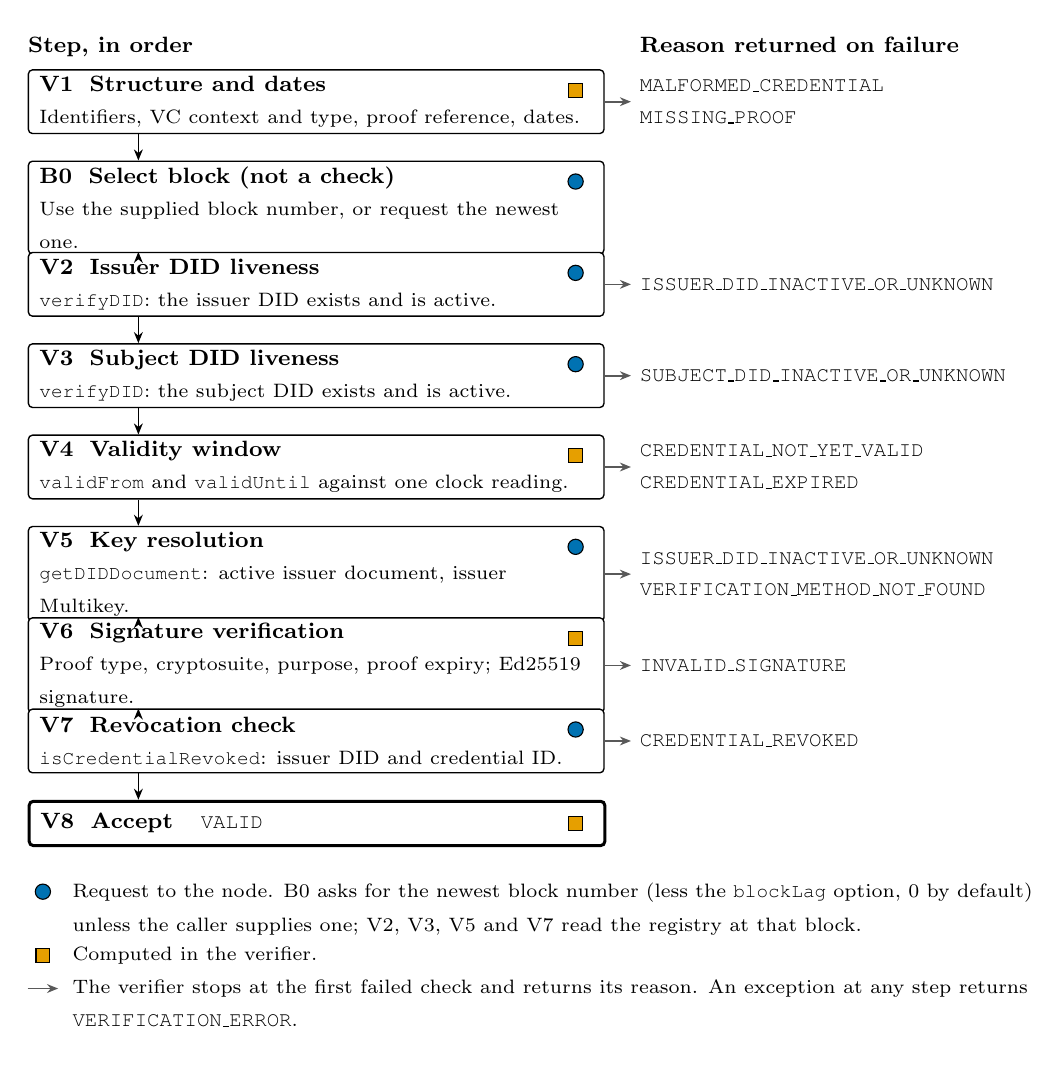
\begin{tikzpicture}[x=1pt,y=1pt,
    stepbox/.style={draw=black, line width=0.5pt, rounded corners=1.5pt, minimum width=208pt,
                 minimum height=23pt, inner xsep=4pt, inner ysep=2pt, anchor=north west,
                 align=flush left, text width=200pt, fill=white},
    flow/.style={-{Stealth[length=4pt,width=3.2pt]}, line width=0.6pt, draw=black},
    fail/.style={-{Stealth[length=4pt,width=3.2pt]}, line width=0.6pt, draw=failgrey},
    nodemark/.style={circle, fill=oiblue, draw=black, line width=0.4pt, minimum size=5.5pt, inner sep=0pt},
    compmark/.style={rectangle, fill=oiorange, draw=black, line width=0.4pt, minimum size=5pt, inner sep=0pt},
  ]
  % Fixed bounding box: 363.2 pt wide (TeX points, as \columnwidth).
  \useasboundingbox (0,0) rectangle (363.2,-366);

  % Column heads
  \node[anchor=base west, inner sep=0pt] at (0,-9) {\fontsize{8}{9.5}\selectfont\bfseries Step, in order};
  \node[anchor=base west, inner sep=0pt] at (221,-9) {\fontsize{8}{9.5}\selectfont\bfseries Reason returned on failure};

  % Pitch 33 pt: box 23 pt, gap 10 pt. First box top at y = -15. Marker at x = 198 on the title line.
  \foreach \i/\mark/\key/\name/\detail in {
      0/compmark/V1/Structure and dates/{Identifiers, VC context and type, proof reference, dates.},
      1/nodemark/B0/Select block (not a check)/{Use the supplied block number, or request the newest one.},
      2/nodemark/V2/Issuer DID liveness/{\fn{verifyDID}: the issuer DID exists and is active.},
      3/nodemark/V3/Subject DID liveness/{\fn{verifyDID}: the subject DID exists and is active.},
      4/compmark/V4/Validity window/{\fn{validFrom} and \fn{validUntil} against one clock reading.},
      5/nodemark/V5/Key resolution/{\fn{getDIDDocument}: active issuer document, issuer Multikey.},
      6/compmark/V6/Signature verification/{Proof type, cryptosuite, purpose, proof expiry; Ed25519 signature.},
      7/nodemark/V7/Revocation check/{\fn{isCredentialRevoked}: issuer DID and credential ID.}%
    }{
    \node[stepbox] (\key) at (0,{-15-\i*33}) {\steptitle{\key}{\name}\\[-0.5pt]\stepdetail{\detail}};
    \node[\mark] at (198,{-15-\i*33-7.6}) {};
  }

  % V8 accept (gap 10 pt below V7)
  \node[stepbox, line width=1.1pt, minimum height=16pt] (V8) at (0,-279)
    {\steptitle{V8}{Accept}\hspace{1em}\code{VALID}};
  \node[compmark] at (198, 0 |- V8.east) {};

  % Flow arrows (pass), 40 pt from the left edge of the boxes
  \foreach \a/\b in {V1/B0,B0/V2,V2/V3,V3/V4,V4/V5,V5/V6,V6/V7,V7/V8}{
    \draw[flow] (40, 0 |- \a.south) -- (40, 0 |- \b.north);
  }

  % Failure arrows and reason codes (right column starts at x = 221)
  \newcommand{\failone}[2]{%
    \draw[fail] (#1.east) -- (218, 0 |- #1.east);
    \node[anchor=west, inner sep=0pt] at (221, 0 |- #1.east) {\code{#2}};}
  \newcommand{\failtwo}[3]{%
    \draw[fail] (#1.east) -- (218, 0 |- #1.east);
    \node[anchor=west, inner sep=0pt, align=flush left] at (221, 0 |- #1.east) {\code{#2}\\[-0.5pt]\code{#3}};}
  \failtwo{V1}{MALFORMED\_CREDENTIAL}{MISSING\_PROOF}
  \failone{V2}{ISSUER\_DID\_INACTIVE\_OR\_UNKNOWN}
  \failone{V3}{SUBJECT\_DID\_INACTIVE\_OR\_UNKNOWN}
  \failtwo{V4}{CREDENTIAL\_NOT\_YET\_VALID}{CREDENTIAL\_EXPIRED}
  \failtwo{V5}{ISSUER\_DID\_INACTIVE\_OR\_UNKNOWN}{VERIFICATION\_METHOD\_NOT\_FOUND}
  \failone{V6}{INVALID\_SIGNATURE}
  \failone{V7}{CREDENTIAL\_REVOKED}

  % Key: three entries, glyph at x = 0 to 11, text from x = 16
  \def\ka{-309} \def\kb{-332} \def\kc{-344}
  \node[nodemark] at (5.5,\ka-3.2) {};
  \node[anchor=north west, inner sep=0pt, text width=347pt, align=flush left] at (16,\ka)
    {\stepdetail{Request to the node. B0 asks for the newest block number (less the \fn{blockLag} option, 0 by default) unless the caller supplies one; V2, V3, V5 and V7 read the registry at that block.}};
  \node[compmark] at (5.5,\kb-3.2) {};
  \node[anchor=north west, inner sep=0pt, text width=347pt, align=flush left] at (16,\kb)
    {\stepdetail{Computed in the verifier.}};
  \draw[fail] (0,\kc-3.2) -- (11,\kc-3.2);
  \node[anchor=north west, inner sep=0pt, text width=347pt, align=flush left] at (16,\kc)
    {\stepdetail{The verifier stops at the first failed check and returns its reason. An exception at any step returns \code{VERIFICATION\_ERROR}.}};
\end{tikzpicture}
\end{document}
